% Chapter7
\chapter{Streaming} \label{chapter:Streaming}
This chapter explains the network structure of the whole project and how the connections between the servers and the app are done.
\subsection{General network}
The following figure shows the detailed network set-up and application flow of the project.
\begin{figure}[htbp]
\centering
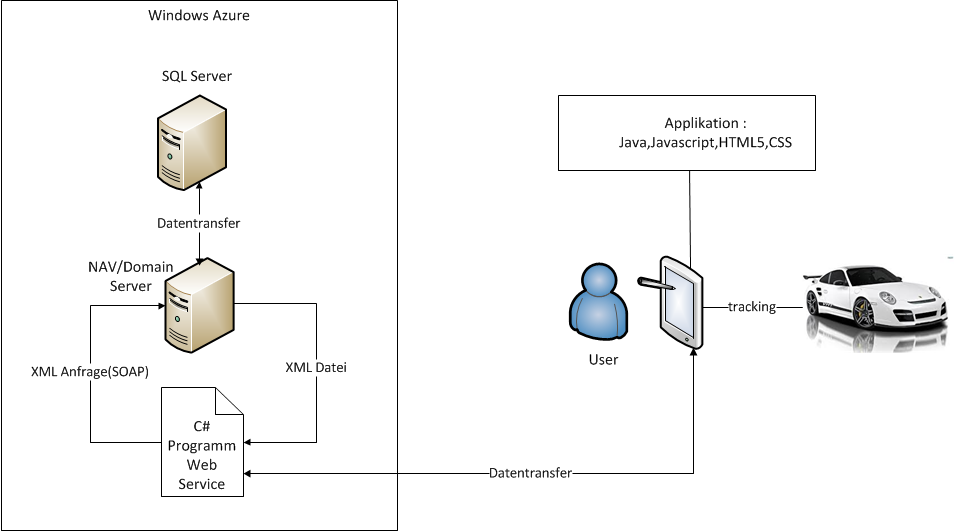
\includegraphics[width=\textwidth,height=\textheight,keepaspectratio]
{graphics/networkoverview.png}
\caption{network overview}
\end{figure}

The front end consists of an application which runs on a mobile device and is operated by a user. On the back end is a Microsoft Windows Azure platform which contains the following two server instances. The server with Microsoft SQL in the top of the graphic is for saving and processing the data. The bottom server in the graphic, the main server on which runs Microsoft NAV 2013 and a domain for communicating with the SQL server. Both of these server operation systems are windows server 2008 R2. The C\# application is installed as a windows service and is used to communicate between back end and front end.

\subsection{C\# Application}
The application consists of two important main parts. The first part is the communication between the NAV server and the C\# program. To solve this problem it uses a NAV web service to access and receive the needed data. The NAV web service will be explained in the following sub chapter ''NAV Server''. When the set up of the NAV web service is done it can be simply added as a web reference in Visual Studio to access it in the code.
\\\\
\begin{description}
   \item[The application has three web references]~\par
   \begin{enumerate}
      \item NavArCarData, which is used to get all information about a tracked car. 
      \item NavArTrackingHistory , which is used to save a history of tracked cars.
      \item	NavArUserData, which is used to save data from the user. 
   \end{enumerate}
\end{description}

\begin{figure}[htbp]
\centering
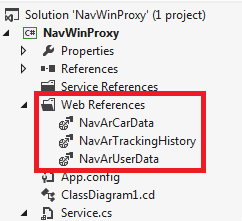
\includegraphics[width=40mm,height=\textheight,keepaspectratio]{graphics/webref.png}
\caption{web reference}
\end{figure}
The web references can be accessed via the code in Visual Studio.
\newpage
\definecolor{bluekeywords}{rgb}{0.13,0.13,1}
\definecolor{greencomments}{rgb}{0,0.5,0}
\definecolor{redstrings}{rgb}{0.9,0,0}
\lstset{language=[Sharp]C,
  breaklines=true,
  commentstyle=\color{greencomments},
  keywordstyle=\color{bluekeywords},
  stringstyle=\color{redstrings}
}
\subsubsection{Read from the web service}
\begin{lstlisting}[caption=Example reading webservice,captionpos=b]
//use the created web reference
using NavWinProxy.NavArCarData;
//Create a service object
NavArCarDataPage_Service service = new NavArCarDataPage_Service();
//set user credentials which have access rights to the NAV server
service.Credentials = System.Net.CredentialCache.DefaultCredentials;
//create a new Object for storing the data
NavArCarDataPage carData = new NavArCarDataPage();                
//read the data which a specific id
carData = service.Read('1');
//check if the id exists
if (carData != null){
   //access data and store data
   string accessData=carData.Feld1;
}
\end{lstlisting}      

In this code example the web reference can simply accessed with the using statement and a service object. After that the credentials are set with ''System.Net.CredentialCache.DefaultCredentials''.
These are the default credentials from the user who runs the program. After that a  NavArCarDataPage object is created for storing data from the web service. Then the data can easily read with service object with service.Read(String ID)  method.
\newpage
\subsubsection{Write to the web service}
\begin{lstlisting}[caption=Example writing to web service,captionpos=b]
 public string insertProfileData(string androidEmail,string profileEmail, string firstName, string lastName, string hash)
        {
        //create the service object
        NavArUserDataPage_Service service = new NavArUserDataPage_Service();
        //set user credentials which have access rights to the NAV server
        service.Credentials = System.Net.CredentialCache.DefaultCredentials;
        //read the user data from a specific google mail address
        NavArUserDataPage userData = service.Read(androidEmail);
        //check if the email exis 
        if (userData != null)
            {
            //set the profile data
            userData.Feld2 = profileEmail;
            userData.Feld3 = firstName;
            userData.Feld4 = lastName;
            //update the nav database with the new data
            service.Update(ref userData);
            }
            else return "fail";
                return "success";
            }
            else return "fail";
        }
\end{lstlisting}
The beginning of the example code is similar to reading from the web service.At line number 8 profile data are read with a google email adress and is checked if it exist. If it exist the attributes for are profile email,first name and last name is set and it get updated with .Update(Object to Update) method.The shown example method is simply used for inserting/updating profile data from the application in the Navsion Server 
  
\newpage
\subsubsection{Provide a web service}

The other important part of this application is to provide a web service for communication with the mobile devices.  To provide the functionality the C\# program uses ''System.Service.Model.web'' which contains several methods for implementing a web service.  In the following code example an operation contract is made to publish specific methods so that the mobile devices can access these methods.
\\\\
\begin{lstlisting}[caption=
ServiceContract,captionpos=b]
[ServiceContract]
    public interface IOrderService
    {
        [OperationContract]
        [WebGet(UriTemplate = "getKFZInfo/{id}/{hash}",ResponseFormat =           
        WebMessageFormat.Json,RequestFormat = WebMessageFormat.Json)]
        string getKFZInfo(string id,string hash);
    }
\end{lstlisting}

This example consist of one method ''getKFZInfo'' with two parameters id and hash. It returns the car information with the given id if the hash is correct. The hash value is used to prevent access from other unwanted programs. The method could be access via the web url ''serveradress/getKFZInfo/id/hashvalue''. An invocation with the web browser would look like this:  127.0.0.1/getKFZInfo/5/ac3rf229f1fb88a8719e5f6d29443545
\newpage
\subsubsection{Communication from mobile device to the C\# App}

The mobile app access the web service of the C\# application within JavaScript. Ajax is used for providing the communication between the user and the server. In the following code example an Ajax request to the server is shown.


\begin{lstlisting}[language=html, caption=readcarname example,captionpos=b]
function readcarname(cname){
        $(document).ready(function () {
            $.ajax({
                type: "GET",
                url: "http://tgm.cloudapp.net:9090/rest/getKFZInfo/"
                +cname+"/ac73f229f1fb88a8719e5f6d295bee45?callback=?"
                ,async: false,
                dataType: 'JSONP',
                success: function(data){
                    globalcarname= data.split(';')[0];
                }
            });
        });
    }
\end{lstlisting}
This example consist of one function readcarname(cname) which sends an Ajax request with a given parameter to the server. The first part of the url in the request represents the azure domain: http://tgm.cloudapp.net:9090 where the C\# application is hosted and the second part is the method which should be called. The dataType is JSONP so that it is possible to transfer and receive data over different domains. The success method in the Ajax request will be triggered after the server sends the data back. In this example the response data from the server is stored in the variable ''globalcarname''.
\newpage
\subsection{NAV Server}
For storing and receiving the important data for the mobile application a NAV Server 2013 is used.
\subsubsection{Table structure}
\begin{description}
   \item[The table structure contains three tables for storing]~\par
   \begin{enumerate}
      \item NavArTrackingHistory 
      \item NavArCarData
      \item	NavArUserData. 
   \end{enumerate}
\end{description}

The NavArTrackingHistory table is used to save the tracking history of a user to the database. It has six columns for saving the tracking history of a user.
\newline
\begin{figure}[htbp]
\centering
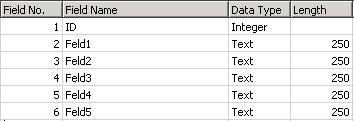
\includegraphics[width=100mm,height=\textheight,keepaspectratio]{graphics/trackingtable.png}
\caption{NavArTtrackingHistory table}
\end{figure}
\newline
  The following figure shows an example entry. This entry consist of a unique ID, email address, ID of the tracked car, start time, end time and duration.  
\begin{figure}[htbp]
\centering
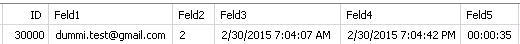
\includegraphics[width=\textwidth,height=\textheight,keepaspectratio]{graphics/trackingtableexample.png}
\caption{Example table entry}
\end{figure}
\newpage
The NavArCarData table stores all necessary information about the available cars which can be tracked.
\begin{figure}[htbp]
\centering
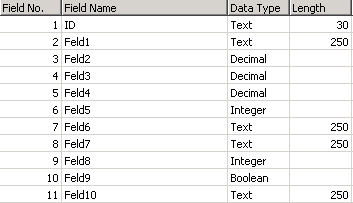
\includegraphics[width=80mm,height=\textheight,keepaspectratio]{graphics/cardatatable.png}
\caption{NavArCarData table}
\end{figure}
\\
The following figure of a entry consists of a unique car ID, car name, car price, leasing car price, monthly leasing price, horse power(hp), engine , motor fuel, number of doors, parking sensors and color. 
\newline  
\begin{figure}[htbp]
\centering
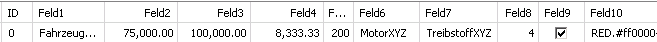
\includegraphics[width=\textwidth,height=\textheight,keepaspectratio]{graphics/cardatatablentry.png}
\caption{Example table entry}
\end{figure}
\newline
The NavArUserData table has four columns which are used for saving the google email address,a custom email address, a name and a surname.
\\\\
\begin{figure}[htbp]
\centering
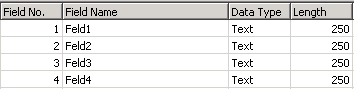
\includegraphics[width=100mm,height=\textheight,keepaspectratio]{graphics/userdatatable.png}
\caption{NavArUserData table }
\end{figure}
\\
\begin{figure}[htbp]
\centering
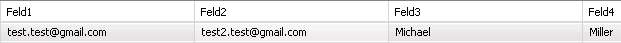
\includegraphics[width=\textwidth,height=\textheight,keepaspectratio]{graphics/userdatatableentry.png}
\caption{Example table entry}
\end{figure}
\newpage
To provide access to these three tables a page for each table was created with the same structure as the tables.  
\subsection{Web service}
The communication between the C\# application and the NAV server was achieved by a web service. The web service functionality is built in the NAV server and can be used to publish pages.A page was published for each of the mentioned tables of the previous chapter. 
\\\\
\begin{figure}[htbp]
\centering
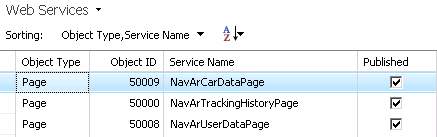
\includegraphics[width=\textwidth,height=\textheight,keepaspectratio]{graphics/webservice.png}
\caption{published pages}
\end{figure}
\\\\
These pages can be accessed via the web service from other programs. The web service also provides methods for creating, reading, deleting and updating data.
An example for reading from and writing to a web service can be found in the chapter Streaming C\# Application.   
\newpage
